\chapter{UMSAP Control}
\label{chap:umsapCtrl}

The UMSAP Control windows shows the content of an umsap file (\autoref{fig:umsapCtrlWin}).

\section{The interface}

The analysis contained in the selected umsap file are displayed in alphabetical
order and grouped by the analysis type. The checkboxes to the left of the names of
the Modules and Utilities allow creating the corresponding window showing the results
available for the selected Module or Utility.

\begin{figure}[h]
    \centering
    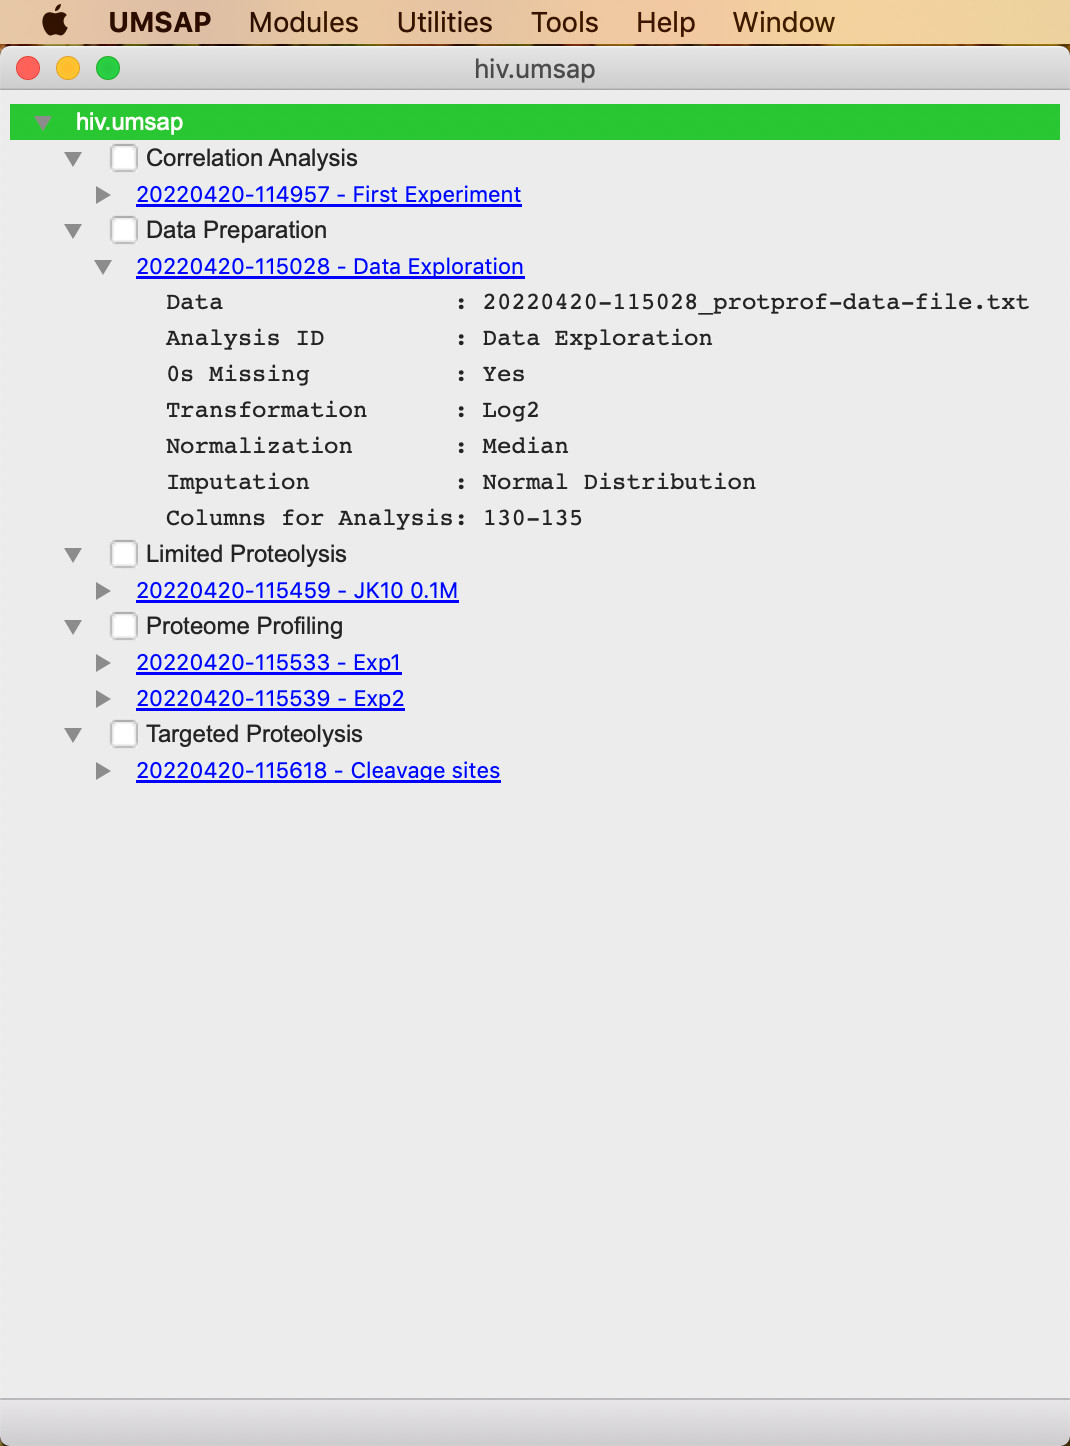
\includegraphics[width=0.7\textwidth]{./IMAGES/UMSAPCtrl/UMSAPCtrl.jpg}
    \caption[The UMSAP Control window]{\textbf{The UMSAP Control window.} The content
    of the selected umsap file is shown in alphabetically order. The window allows
    managing the content of the umsap file and to visualize the results of the analysis
    in the file.} 
    \label{fig:umsapCtrlWin}
    \vspace{-5pt}
\end{figure}

Each analysis in the file is represented by the user-provided Analysis ID. Unfolding
any ID will display all the configuration values provided by the user prior to running
the analysis. In addition, a left click over any Analysis ID will create the corresponding
tab in the Analysis Setup window (\autoref{fig:mainWindow}) and populate all fields
with the values in the selected analysis. This is the fastest way to configure the
analysis tab to rerun an analysis with slight changes in the configuration options.
After rerunning an analysis or simply adding a new analysis to the umsap file, the
window will be automatically updated to incorporate the new results.

\section{The Tools menu}

The UMSAP Control windows also allows managing the content of the selected umsap
file. Currently, it is possible to Add (Cmd+A) analysis from a different umsap
file, to Delete (Cmd+X) analysis from an existing umsap file and to Export (Cmd+E)
the analysis in an umsap file to a new umsap file.

Adding analysis from an umsap file to the already opened umsap file will result
in the addition of the new information to the already opened umsap file and in the
copy of the necessary files and folders to folders Input{\_}Data{\_}Files and
Steps{\_}Data{\_}Files. During this process there is a small chance to end up with
duplicated file and/or folder names or Analysis ID. In this case, UMSAP will rename
the file/folder/Analysis ID to avoid any overwriting and will update any reference
in the umsap file to the files/folders that were renamed.

Deleting any analysis from an umsap file will also result in the removal of the
files and/or folders referenced in the deleted analysis. Files in Input{\_}Data{\_}Files
are only deleted if they are not referenced by any remaining analysis. Deleting
all analysis in an umsap file will result in the removal of the umsap file and folders
Input{\_}Data{\_}Files and Steps{\_}Data{\_}Files. If the folder containing the
project is empty after deleting all UMSAP files and folders the project folder is
also deleted.

Exporting some or all analysis in an opened umsap file to an already existing umsap
file is not possible. When exporting the selected analysis to a project folder containing
an Input{\_}Data{\_}Files and/or Steps{\_}Data{\_}Files folder, UMSAP will create a new
folder in the selected project folder and export all the information to this empty
folder.


